\subsubsection{Case analysis of the live Lean state}
\label{subsec:barrel-live-state-cases}

The infoview panel exposes the same refinement-chain experiment while it is
running and while proofs are being edited.  Its states distinguish four cases
which matter operationally: an import still in progress; an incomplete proof
skeleton; a complete script containing admissions; and an admission-free
completion.  The figures below redraw the actual interface in TikZ so that its
geometry, colors, and typography remain reproducible in the manuscript.

\definecolor{barrelUiBackground}{RGB}{253,248,237}
\definecolor{barrelUiBorder}{RGB}{209,215,208}
\definecolor{barrelUiAuto}{RGB}{105,198,143}
\definecolor{barrelUiHand}{RGB}{7,183,208}
\definecolor{barrelUiSorry}{RGB}{219,153,69}
\definecolor{barrelUiPending}{RGB}{200,209,203}
\definecolor{barrelUiPale}{RGB}{184,217,219}
\definecolor{barrelUiText}{RGB}{0,82,96}
\definecolor{barrelUiLabel}{RGB}{70,123,132}
\definecolor{barrelUiMuted}{RGB}{124,158,163}
\definecolor{barrelUiLegendAuto}{RGB}{164,214,177}
\definecolor{barrelUiLegendHand}{RGB}{104,202,217}
\definecolor{barrelUiLegendSorry}{RGB}{236,178,105}
\definecolor{barrelUiLegendPending}{RGB}{213,219,213}
\definecolor{barrelUiError}{RGB}{196,71,31}
\definecolor{barrelUiBarrel}{RGB}{224,157,35}
\definecolor{barrelUiBarrelDark}{RGB}{87,53,9}

\paragraph*{Loading and pending.}
As soon as an artifact is registered, its card exists even though the final
number of translated goals may still change.  A grey disc denotes such a
pending state; the animated barrel marks the artifact currently being
processed.  The filled part of each bar records obligations whose automatic
attempt has finished, while the pale tail is work not yet processed.  In
\Cref{fig:barrel-state-loading}, \texttt{MinSearch} has reached six of seven
goals and \texttt{MinSearch\_r1} is still importing at twenty-three of
twenty-nine.

\begin{figure}[ht!]
  \centering
  \tikzsetnextfilename{barrel-state-loading}
  \resizebox{\textwidth}{!}{%
    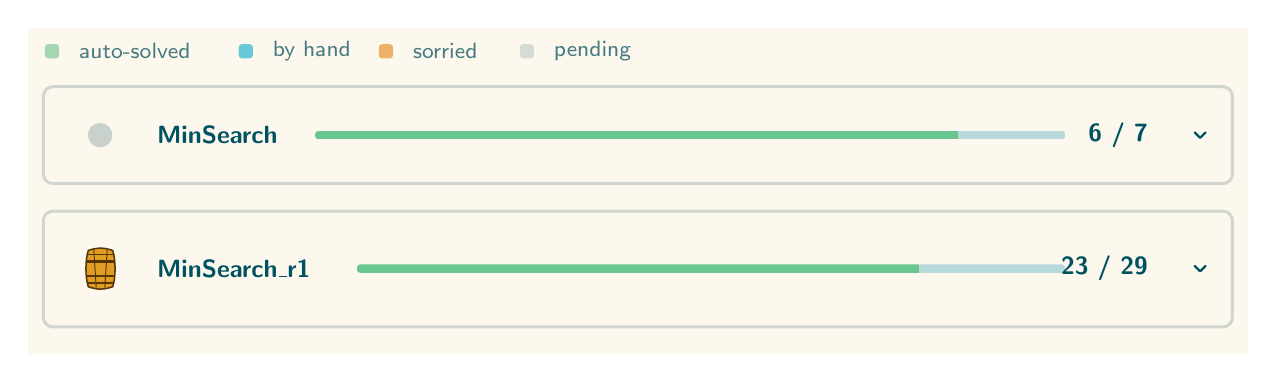
\begin{tikzpicture}[x=1cm,y=1cm,
      legend/.style={font=\fontsize{8.4}{9.4}\selectfont\sffamily,
        text=barrelUiLabel, anchor=west},
      machine/.style={font=\fontsize{9.0}{10}\selectfont\sffamily\bfseries,
        text=barrelUiText, anchor=west},
      meta/.style={font=\fontsize{9.0}{10}\selectfont\sffamily\bfseries,
        text=barrelUiText, anchor=east},
      card/.style={draw=barrelUiBorder, fill=barrelUiBackground,
        rounded corners=.12cm, line width=1.1pt}]
      \useasboundingbox (0,0) rectangle (15.5,4.15);
      \fill[barrelUiBackground] (0,0) rectangle (15.5,4.15);

      \path[fill=barrelUiLegendAuto, rounded corners=.04cm]
        (.22,3.76) rectangle ++(.18,.18);
      \node[legend] at (.53,3.85) {auto-solved};
      \path[fill=barrelUiLegendHand, rounded corners=.04cm]
        (2.68,3.76) rectangle ++(.18,.18);
      \node[legend] at (2.99,3.85) {by hand};
      \path[fill=barrelUiLegendSorry, rounded corners=.04cm]
        (4.46,3.76) rectangle ++(.18,.18);
      \node[legend] at (4.77,3.85) {sorried};
      \path[fill=barrelUiLegendPending, rounded corners=.04cm]
        (6.25,3.76) rectangle ++(.18,.18);
      \node[legend] at (6.56,3.85) {pending};

      \path[card] (.20,2.17) rectangle (15.30,3.40);
      \fill[barrelUiPending] (.92,2.785) circle (.155);
      \node[machine] at (1.52,2.785) {MinSearch};
      \begin{scope}
        \clip[rounded corners=.045cm] (3.65,2.73) rectangle (13.18,2.84);
        \fill[barrelUiAuto] (3.65,2.73) rectangle (11.82,2.84);
        \fill[barrelUiPale] (11.82,2.73) rectangle (13.18,2.84);
      \end{scope}
      \node[meta] at (14.35,2.785) {6 / 7};
      \draw[barrelUiText, line width=.8pt, line cap=round, line join=round]
        (14.82,2.82) -- (14.89,2.75) -- (14.96,2.82);

      \path[card] (.20,.35) rectangle (15.30,1.82);
      % Vector barrel used in the live loading slot.
      \path[fill=barrelUiBarrel, draw=barrelUiBarrelDark, line width=.55pt]
        (.77,.86) .. controls (.73,.98) and (.73,1.20) .. (.77,1.32)
        .. controls (.88,1.36) and (.97,1.36) .. (1.08,1.32)
        .. controls (1.12,1.20) and (1.12,.98) .. (1.08,.86)
        .. controls (.97,.82) and (.88,.82) .. cycle;
      \draw[barrelUiBarrelDark, line width=.55pt] (.77,1.27) -- (1.08,1.27);
      \draw[barrelUiBarrelDark, line width=.8pt] (.75,1.18) -- (1.10,1.18);
      \draw[barrelUiBarrelDark, line width=.8pt] (.75,1.00) -- (1.10,1.00);
      \draw[barrelUiBarrelDark, line width=.55pt] (.77,.91) -- (1.08,.91);
      \draw[barrelUiBarrelDark, line width=.35pt] (.87,.85) -- (.84,1.33);
      \draw[barrelUiBarrelDark, line width=.35pt] (.98,.85) -- (1.01,1.33);

      \node[machine] at (1.52,1.09) {MinSearch\_r1};
      \begin{scope}
        \clip[rounded corners=.045cm] (4.18,1.035) rectangle (13.18,1.145);
        \fill[barrelUiAuto] (4.18,1.035) rectangle (11.32,1.145);
        \fill[barrelUiPale] (11.32,1.035) rectangle (13.18,1.145);
      \end{scope}
      \node[meta] at (14.35,1.09) {23 / 29};
      \draw[barrelUiText, line width=.8pt, line cap=round, line join=round]
        (14.82,1.125) -- (14.89,1.055) -- (14.96,1.125);
    \end{tikzpicture}%
  }
  \caption{The live state while \texttt{MinSearch\_r1} is loading.  The
    status symbols and pale bar segments denote work whose final state is not
    yet known.}
  \label{fig:barrel-state-loading}
\end{figure}
\FloatBarrier

\paragraph*{Missing proof blocks.}
After import, the panel knows the final goal map.  If fewer
\texttt{next} blocks are present than required, the card displays a red cross
and the absent goals remain grey.  The numerator counts proved obligations, so
the state in \Cref{fig:barrel-state-missing} is at $27/29$.  The
\emph{+ proof skeleton} action is available precisely in this case and inserts
the two missing named blocks; it is an editor action, not a proof step.

\begin{figure}[ht!]
  \centering
  \tikzsetnextfilename{barrel-state-missing}
  \resizebox{\textwidth}{!}{%
    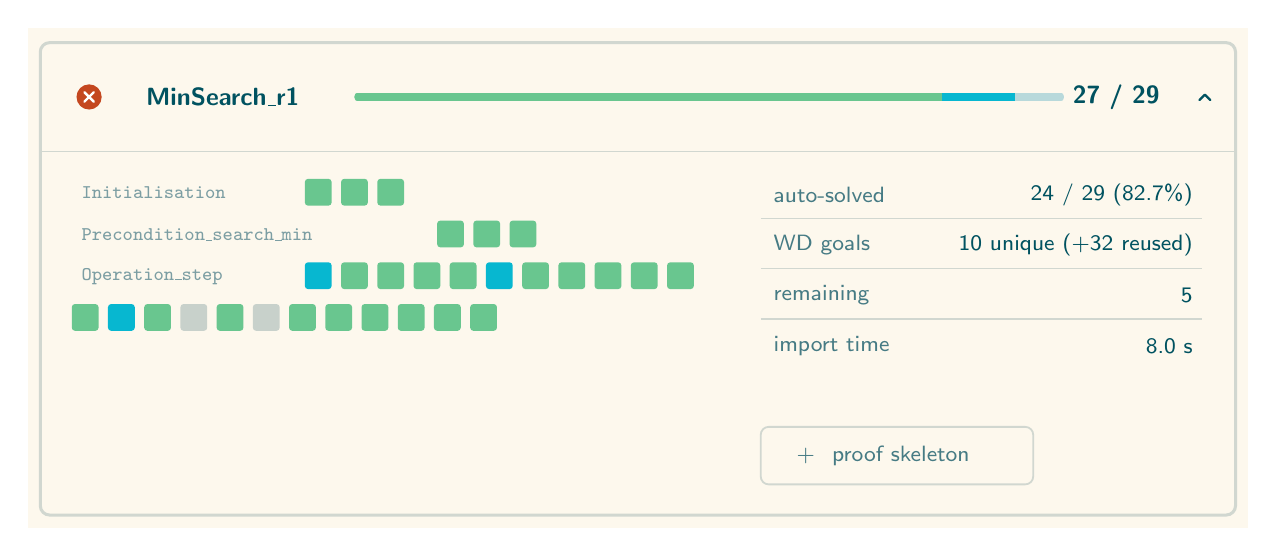
\begin{tikzpicture}[x=1cm,y=1cm,
      machine/.style={font=\fontsize{8.8}{9.8}\selectfont\sffamily\bfseries,
        text=barrelUiText, anchor=west},
      meta/.style={font=\fontsize{8.8}{9.8}\selectfont\sffamily\bfseries,
        text=barrelUiText, anchor=east},
      operation/.style={font=\fontsize{7.2}{8.2}\selectfont\ttfamily,
        text=barrelUiMuted, anchor=west},
      stat/.style={font=\fontsize{7.7}{8.7}\selectfont\sffamily,
        text=barrelUiLabel, anchor=west},
      value/.style={font=\fontsize{7.7}{8.7}\selectfont\sffamily,
        text=barrelUiText, anchor=east},
      card/.style={draw=barrelUiBorder, fill=barrelUiBackground,
        rounded corners=.12cm, line width=1.1pt},
      divider/.style={draw=barrelUiBorder, line width=.5pt}]
      \useasboundingbox (0,0) rectangle (15.5,6.35);
      \fill[barrelUiBackground] (0,0) rectangle (15.5,6.35);
      \path[card] (.16,.16) rectangle (15.34,6.16);
      \draw[divider] (.16,4.78) -- (15.34,4.78);

      \fill[barrelUiError] (.78,5.47) circle (.16);
      \draw[white, line width=.85pt, line cap=round]
        (.72,5.41) -- (.84,5.53) (.72,5.53) -- (.84,5.41);
      \node[machine] at (1.38,5.47) {MinSearch\_r1};
      \begin{scope}
        \clip[rounded corners=.045cm] (4.15,5.415) rectangle (13.16,5.525);
        \fill[barrelUiAuto] (4.15,5.415) rectangle (11.61,5.525);
        \fill[barrelUiHand] (11.61,5.415) rectangle (12.54,5.525);
        \fill[barrelUiPale] (12.54,5.415) rectangle (13.16,5.525);
      \end{scope}
      \node[meta] at (14.50,5.47) {27 / 29};
      \draw[barrelUiText, line width=.8pt, line cap=round, line join=round]
        (14.88,5.43) -- (14.95,5.50) -- (15.02,5.43);

      \node[operation] at (.56,4.25) {Initialisation};
      \foreach[count=\i from 0] \c in {barrelUiAuto,barrelUiAuto,barrelUiAuto}{
        \path[fill=\c, rounded corners=.04cm]
          ({3.52+.46*\i},4.09) rectangle ++(.34,.34);}
      \node[operation] at (.56,3.72) {Precondition\_search\_min};
      \foreach[count=\i from 0] \c in {barrelUiAuto,barrelUiAuto,barrelUiAuto}{
        \path[fill=\c, rounded corners=.04cm]
          ({5.20+.46*\i},3.56) rectangle ++(.34,.34);}
      \node[operation] at (.56,3.19) {Operation\_step};
      \foreach[count=\i from 0] \c in {
          barrelUiHand,barrelUiAuto,barrelUiAuto,barrelUiAuto,barrelUiAuto,
          barrelUiHand,barrelUiAuto,barrelUiAuto,barrelUiAuto,barrelUiAuto,
          barrelUiAuto}{
        \path[fill=\c, rounded corners=.04cm]
          ({3.52+.46*\i},3.03) rectangle ++(.34,.34);}
      \foreach[count=\i from 0] \c in {
          barrelUiAuto,barrelUiHand,barrelUiAuto,barrelUiPending,
          barrelUiAuto,barrelUiPending,barrelUiAuto,barrelUiAuto,
          barrelUiAuto,barrelUiAuto,barrelUiAuto,barrelUiAuto}{
        \path[fill=\c, rounded corners=.04cm]
          ({.56+.46*\i},2.50) rectangle ++(.34,.34);}

      \node[stat] at (9.35,4.23) {auto-solved};
      \node[value] at (14.92,4.23) {24 / 29 (82.7\%)};
      \draw[divider] (9.31,3.93) -- (14.92,3.93);
      \node[stat] at (9.35,3.59) {WD goals};
      \node[value] at (14.92,3.59) {10 unique (+32 reused)};
      \draw[divider] (9.31,3.29) -- (14.92,3.29);
      \node[stat] at (9.35,2.95) {remaining};
      \node[value] at (14.92,2.95) {5};
      \draw[divider] (9.31,2.65) -- (14.92,2.65);
      \node[stat] at (9.35,2.31) {import time};
      \node[value] at (14.92,2.31) {8.0 s};

      \path[draw=barrelUiBorder, fill=barrelUiBackground,
        rounded corners=.10cm, line width=.65pt]
        (9.31,.55) rectangle (12.77,1.28);
      \node[font=\fontsize{8.0}{9.0}\selectfont\sffamily,
        text=barrelUiLabel, anchor=west] at (9.64,.915)
        {+\hspace{.22cm}proof skeleton};
    \end{tikzpicture}%
  }
  \caption{An expanded card with two missing proof blocks.  Grey cells mark
    the missing goals and the proof-skeleton action mirrors the button shown by
    Lean.}
  \label{fig:barrel-state-missing}
\end{figure}
\FloatBarrier

\paragraph*{Admitted goals.}
A script may contain the required number of blocks yet use \texttt{sorry} in
some of them.  Such blocks are not pending: they occupy their positions in the
script, so the skeleton action disappears.  They are nevertheless excluded
from the proved numerator and are rendered in orange, both in the status slot
and in the operation map.  \Cref{fig:barrel-state-sorry} differs from the
previous state only by replacing its two missing goals with admissions; this
visual distinction prevents a syntactically complete proof script from being
mistaken for an admission-free development.

\begin{figure}[ht!]
  \centering
  \tikzsetnextfilename{barrel-state-sorry}
  \resizebox{\textwidth}{!}{%
    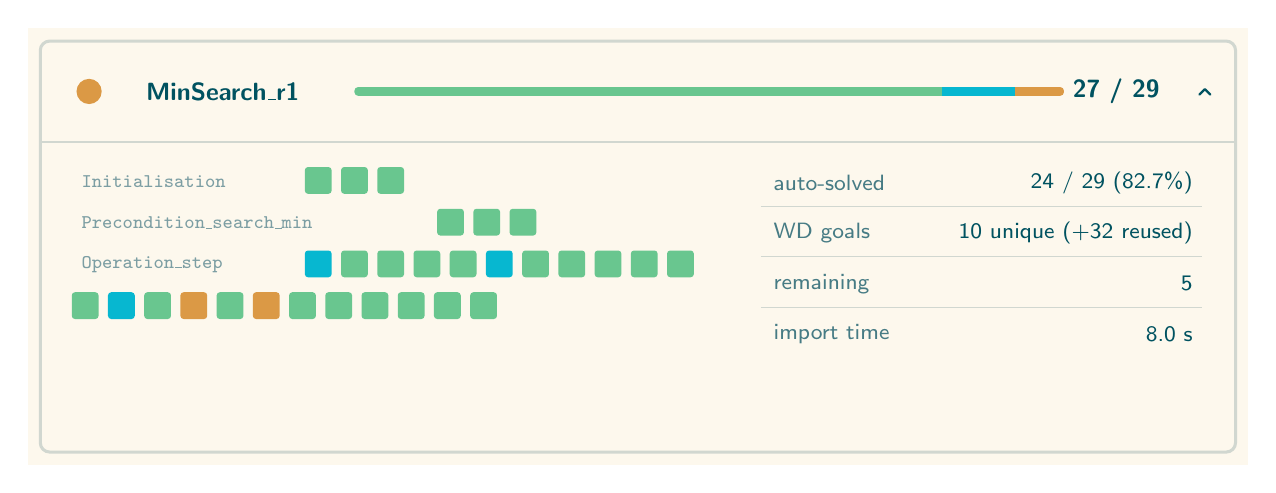
\begin{tikzpicture}[x=1cm,y=1cm,
      machine/.style={font=\fontsize{8.8}{9.8}\selectfont\sffamily\bfseries,
        text=barrelUiText, anchor=west},
      meta/.style={font=\fontsize{8.8}{9.8}\selectfont\sffamily\bfseries,
        text=barrelUiText, anchor=east},
      operation/.style={font=\fontsize{7.2}{8.2}\selectfont\ttfamily,
        text=barrelUiMuted, anchor=west},
      stat/.style={font=\fontsize{7.7}{8.7}\selectfont\sffamily,
        text=barrelUiLabel, anchor=west},
      value/.style={font=\fontsize{7.7}{8.7}\selectfont\sffamily,
        text=barrelUiText, anchor=east},
      card/.style={draw=barrelUiBorder, fill=barrelUiBackground,
        rounded corners=.12cm, line width=1.1pt},
      divider/.style={draw=barrelUiBorder, line width=.5pt}]
      \useasboundingbox (0,0) rectangle (15.5,5.55);
      \fill[barrelUiBackground] (0,0) rectangle (15.5,5.55);
      \path[card] (.16,.16) rectangle (15.34,5.38);
      \draw[divider] (.16,4.10) -- (15.34,4.10);

      \fill[barrelUiSorry] (.78,4.74) circle (.16);
      \node[machine] at (1.38,4.74) {MinSearch\_r1};
      \begin{scope}
        \clip[rounded corners=.045cm] (4.15,4.685) rectangle (13.16,4.795);
        \fill[barrelUiAuto] (4.15,4.685) rectangle (11.61,4.795);
        \fill[barrelUiHand] (11.61,4.685) rectangle (12.54,4.795);
        \fill[barrelUiSorry] (12.54,4.685) rectangle (13.16,4.795);
      \end{scope}
      \node[meta] at (14.50,4.74) {27 / 29};
      \draw[barrelUiText, line width=.8pt, line cap=round, line join=round]
        (14.88,4.70) -- (14.95,4.77) -- (15.02,4.70);

      \node[operation] at (.56,3.60) {Initialisation};
      \foreach[count=\i from 0] \c in {barrelUiAuto,barrelUiAuto,barrelUiAuto}{
        \path[fill=\c, rounded corners=.04cm]
          ({3.52+.46*\i},3.44) rectangle ++(.34,.34);}
      \node[operation] at (.56,3.07) {Precondition\_search\_min};
      \foreach[count=\i from 0] \c in {barrelUiAuto,barrelUiAuto,barrelUiAuto}{
        \path[fill=\c, rounded corners=.04cm]
          ({5.20+.46*\i},2.91) rectangle ++(.34,.34);}
      \node[operation] at (.56,2.54) {Operation\_step};
      \foreach[count=\i from 0] \c in {
          barrelUiHand,barrelUiAuto,barrelUiAuto,barrelUiAuto,barrelUiAuto,
          barrelUiHand,barrelUiAuto,barrelUiAuto,barrelUiAuto,barrelUiAuto,
          barrelUiAuto}{
        \path[fill=\c, rounded corners=.04cm]
          ({3.52+.46*\i},2.38) rectangle ++(.34,.34);}
      \foreach[count=\i from 0] \c in {
          barrelUiAuto,barrelUiHand,barrelUiAuto,barrelUiSorry,
          barrelUiAuto,barrelUiSorry,barrelUiAuto,barrelUiAuto,
          barrelUiAuto,barrelUiAuto,barrelUiAuto,barrelUiAuto}{
        \path[fill=\c, rounded corners=.04cm]
          ({.56+.46*\i},1.85) rectangle ++(.34,.34);}

      \node[stat] at (9.35,3.58) {auto-solved};
      \node[value] at (14.92,3.58) {24 / 29 (82.7\%)};
      \draw[divider] (9.31,3.28) -- (14.92,3.28);
      \node[stat] at (9.35,2.94) {WD goals};
      \node[value] at (14.92,2.94) {10 unique (+32 reused)};
      \draw[divider] (9.31,2.64) -- (14.92,2.64);
      \node[stat] at (9.35,2.30) {remaining};
      \node[value] at (14.92,2.30) {5};
      \draw[divider] (9.31,2.00) -- (14.92,2.00);
      \node[stat] at (9.35,1.66) {import time};
      \node[value] at (14.92,1.66) {8.0 s};
    \end{tikzpicture}%
  }
  \caption{The same expanded card after the two missing goals have been
    filled with \texttt{sorry}.  Orange cells identify admissions and the
    insertion action is no longer present.}
  \label{fig:barrel-state-sorry}
\end{figure}
\FloatBarrier

\paragraph*{Admission-free completion.}
Once all obligations have checked proofs, the status becomes a green check and
every card can be collapsed to a one-line project overview.  Expanding a card
retains the operation-level map and the import statistics.  The final
\texttt{MinSearch\_r2} state in \Cref{fig:barrel-state-complete} makes the
post-paper improvements visible together: 47 distinct goals are displayed,
26 were automatic, 21 were proved by hand, and 74 repeated WD occurrences were
resolved by theorem reuse rather than added to the map.

\begin{figure}[ht!]
  \centering
  \tikzsetnextfilename{barrel-state-complete}
  \resizebox{\textwidth}{!}{%
    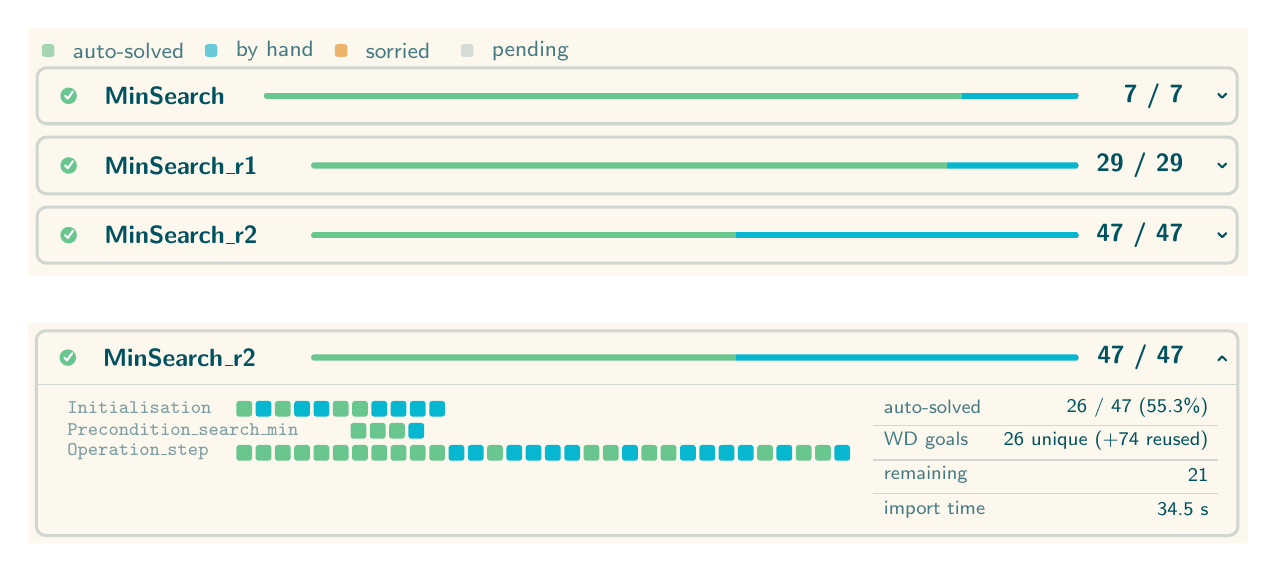
\begin{tikzpicture}[x=1cm,y=1cm,
      legend/.style={font=\fontsize{8.3}{9.3}\selectfont\sffamily,
        text=barrelUiLabel, anchor=west},
      machine/.style={font=\fontsize{8.8}{9.8}\selectfont\sffamily\bfseries,
        text=barrelUiText, anchor=west},
      meta/.style={font=\fontsize{8.8}{9.8}\selectfont\sffamily\bfseries,
        text=barrelUiText, anchor=east},
      operation/.style={font=\fontsize{7.2}{8.2}\selectfont\ttfamily,
        text=barrelUiMuted, anchor=west},
      stat/.style={font=\fontsize{7.3}{8.4}\selectfont\sffamily,
        text=barrelUiLabel, anchor=west},
      value/.style={font=\fontsize{7.3}{8.4}\selectfont\sffamily,
        text=barrelUiText, anchor=east},
      card/.style={draw=barrelUiBorder, fill=barrelUiBackground,
        rounded corners=.12cm, line width=1.1pt},
      divider/.style={draw=barrelUiBorder, line width=.45pt}]
      \useasboundingbox (0,0) rectangle (15.5,6.55);

      % Complete panel with all imported artifacts collapsed.
      \fill[barrelUiBackground] (0,3.40) rectangle (15.5,6.55);
      \path[fill=barrelUiLegendAuto, rounded corners=.035cm]
        (.18,6.18) rectangle ++(.16,.16);
      \node[legend] at (.45,6.26) {auto-solved};
      \path[fill=barrelUiLegendHand, rounded corners=.035cm]
        (2.25,6.18) rectangle ++(.16,.16);
      \node[legend] at (2.52,6.26) {by hand};
      \path[fill=barrelUiLegendSorry, rounded corners=.035cm]
        (3.90,6.18) rectangle ++(.16,.16);
      \node[legend] at (4.17,6.26) {sorried};
      \path[fill=barrelUiLegendPending, rounded corners=.035cm]
        (5.50,6.18) rectangle ++(.16,.16);
      \node[legend] at (5.77,6.26) {pending};

      \foreach \bottom/\top/\cy in {
          5.33/6.04/5.685,4.44/5.16/4.80,3.56/4.27/3.915}{
        \path[card] (.12,\bottom) rectangle (15.36,\top);
        \fill[barrelUiAuto] (.52,\cy) circle (.105);
        \draw[white, line width=.75pt, line cap=round, line join=round]
          (.475,\cy) -- (.51,{\cy-.035}) -- (.575,{\cy+.055});
        \draw[barrelUiText, line width=.75pt, line cap=round, line join=round]
          (15.12,{\cy+.025}) -- (15.17,{\cy-.025}) --
          (15.22,{\cy+.025});}

      \node[machine] at (.85,5.685) {MinSearch};
      \begin{scope}
        \clip[rounded corners=.035cm] (3.00,5.645) rectangle (13.35,5.725);
        \fill[barrelUiAuto] (3.00,5.645) rectangle (11.87,5.725);
        \fill[barrelUiHand] (11.87,5.645) rectangle (13.35,5.725);
      \end{scope}
      \node[meta] at (14.80,5.685) {7 / 7};

      \node[machine] at (.85,4.80) {MinSearch\_r1};
      \begin{scope}
        \clip[rounded corners=.035cm] (3.60,4.76) rectangle (13.35,4.84);
        \fill[barrelUiAuto] (3.60,4.76) rectangle (11.67,4.84);
        \fill[barrelUiHand] (11.67,4.76) rectangle (13.35,4.84);
      \end{scope}
      \node[meta] at (14.80,4.80) {29 / 29};

      \node[machine] at (.85,3.915) {MinSearch\_r2};
      \begin{scope}
        \clip[rounded corners=.035cm] (3.60,3.875) rectangle (13.35,3.955);
        \fill[barrelUiAuto] (3.60,3.875) rectangle (8.99,3.955);
        \fill[barrelUiHand] (8.99,3.875) rectangle (13.35,3.955);
      \end{scope}
      \node[meta] at (14.80,3.915) {47 / 47};

      % The same panel with MinSearch_r2 expanded.
      \fill[barrelUiBackground] (0,0) rectangle (15.5,2.80);
      \path[card] (.11,.10) rectangle (15.37,2.70);
      \draw[divider] (.11,2.02) -- (15.37,2.02);

      \fill[barrelUiAuto] (.51,2.36) circle (.105);
      \draw[white, line width=.75pt, line cap=round, line join=round]
        (.465,2.36) -- (.50,2.325) -- (.565,2.415);
      \node[machine] at (.83,2.36) {MinSearch\_r2};
      \begin{scope}
        \clip[rounded corners=.035cm] (3.60,2.32) rectangle (13.35,2.40);
        \fill[barrelUiAuto] (3.60,2.32) rectangle (8.99,2.40);
        \fill[barrelUiHand] (8.99,2.32) rectangle (13.35,2.40);
      \end{scope}
      \node[meta] at (14.81,2.36) {47 / 47};
      \draw[barrelUiText, line width=.75pt, line cap=round, line join=round]
        (15.12,2.325) -- (15.17,2.375) -- (15.22,2.325);

      \node[operation] at (.38,1.73) {Initialisation};
      \foreach[count=\i from 0] \c in {
          barrelUiAuto,barrelUiHand,barrelUiAuto,barrelUiHand,
          barrelUiHand,barrelUiAuto,barrelUiAuto,barrelUiHand,
          barrelUiHand,barrelUiHand,barrelUiHand}{
        \path[fill=\c, rounded corners=.035cm]
          ({2.65+.245*\i},1.61) rectangle ++(.20,.20);}
      \node[operation] at (.38,1.45) {Precondition\_search\_min};
      \foreach[count=\i from 0] \c in {
          barrelUiAuto,barrelUiAuto,barrelUiAuto,barrelUiHand}{
        \path[fill=\c, rounded corners=.035cm]
          ({4.10+.245*\i},1.33) rectangle ++(.20,.20);}
      \node[operation] at (.38,1.17) {Operation\_step};
      \foreach[count=\i from 0] \c in {
          barrelUiAuto,barrelUiAuto,barrelUiAuto,barrelUiAuto,
          barrelUiAuto,barrelUiAuto,barrelUiAuto,barrelUiAuto,
          barrelUiAuto,barrelUiAuto,barrelUiAuto,barrelUiHand,
          barrelUiHand,barrelUiAuto,barrelUiHand,barrelUiHand,
          barrelUiHand,barrelUiHand,barrelUiAuto,barrelUiAuto,
          barrelUiHand,barrelUiAuto,barrelUiAuto,barrelUiHand,
          barrelUiHand,barrelUiHand,barrelUiHand,barrelUiAuto,
          barrelUiHand,barrelUiAuto,barrelUiAuto,barrelUiHand}{
        \path[fill=\c, rounded corners=.035cm]
          ({2.65+.245*\i},1.05) rectangle ++(.20,.20);}

      \node[stat] at (10.75,1.73) {auto-solved};
      \node[value] at (15.12,1.73) {26 / 47 (55.3\%)};
      \draw[divider] (10.73,1.50) -- (15.12,1.50);
      \node[stat] at (10.75,1.30) {WD goals};
      \node[value] at (15.12,1.30) {26 unique (+74 reused)};
      \draw[divider] (10.73,1.06) -- (15.12,1.06);
      \node[stat] at (10.75,.87) {remaining};
      \node[value] at (15.12,.87) {21};
      \draw[divider] (10.73,.63) -- (15.12,.63);
      \node[stat] at (10.75,.43) {import time};
      \node[value] at (15.12,.43) {34.5 s};
    \end{tikzpicture}%
  }
  \caption{Admission-free completion of the refinement chain: the three
    artifacts collapsed (top), and the completed \texttt{MinSearch\_r2} card
    expanded (bottom).}
  \label{fig:barrel-state-complete}
\end{figure}
\FloatBarrier

The panel is deliberately not part of the proof state.  It reads immutable
progress summaries and source locations from the elaborator service; the
theorems themselves are still created by the discharger and checked by the
kernel.  Consequently the graphical case distinction improves feedback and
proof maintenance without changing the trust boundary, and the same imports
remain usable in non-interactive builds.

\FloatBarrier
